
%% bare_jrnl.tex
%% V1.4b
%% 2015/08/26
%% by Michael Shell
%% see http://www.michaelshell.org/
%% for current contact information.
%%
%% This is a skeleton file demonstrating the use of IEEEtran.cls
%% (requires IEEEtran.cls version 1.8b or later) with an IEEE
%% journal paper.
%%
%% Support sites:
%% http://www.michaelshell.org/tex/ieeetran/
%% http://www.ctan.org/pkg/ieeetran
%% and
%% http://www.ieee.org/

%%*************************************************************************
%% Legal Notice:
%% This code is offered as-is without any warranty either expressed or
%% implied; without even the implied warranty of MERCHANTABILITY or
%% FITNESS FOR A PARTICULAR PURPOSE! 
%% User assumes all risk.
%% In no event shall the IEEE or any contributor to this code be liable for
%% any damages or losses, including, but not limited to, incidental,
%% consequential, or any other damages, resulting from the use or misuse
%% of any information contained here.
%%
%% All comments are the opinions of their respective authors and are not
%% necessarily endorsed by the IEEE.
%%
%% This work is distributed under the LaTeX Project Public License (LPPL)
%% ( http://www.latex-project.org/ ) version 1.3, and may be freely used,
%% distributed and modified. A copy of the LPPL, version 1.3, is included
%% in the base LaTeX documentation of all distributions of LaTeX released
%% 2003/12/01 or later.
%% Retain all contribution notices and credits.
%% ** Modified files should be clearly indicated as such, including  **
%% ** renaming them and changing author support contact information. **
%%*************************************************************************


% *** Authors should verify (and, if needed, correct) their LaTeX system  ***
% *** with the testflow diagnostic prior to trusting their LaTeX platform ***
% *** with production work. The IEEE's font choices and paper sizes can   ***
% *** trigger bugs that do not appear when using other class files.       ***                          ***
% The testflow support page is at:
% http://www.michaelshell.org/tex/testflow/



\documentclass[journal]{IEEEtran}
%
% If IEEEtran.cls has not been installed into the LaTeX system files,
% manually specify the path to it like:
% \documentclass[journal]{../sty/IEEEtran}





% Some very useful LaTeX packages include:
% (uncomment the ones you want to load)


% *** MISC UTILITY PACKAGES ***
%
%\usepackage{ifpdf}
% Heiko Oberdiek's ifpdf.sty is very useful if you need conditional
% compilation based on whether the output is pdf or dvi.
% usage:
% \ifpdf
%   % pdf code
% \else
%   % dvi code
% \fi
% The latest version of ifpdf.sty can be obtained from:
% http://www.ctan.org/pkg/ifpdf
% Also, note that IEEEtran.cls V1.7 and later provides a builtin
% \ifCLASSINFOpdf conditional that works the same way.
% When switching from latex to pdflatex and vice-versa, the compiler may
% have to be run twice to clear warning/error messages.






% *** CITATION PACKAGES ***
%
%\usepackage{cite}
% cite.sty was written by Donald Arseneau
% V1.6 and later of IEEEtran pre-defines the format of the cite.sty package
% \cite{} output to follow that of the IEEE. Loading the cite package will
% result in citation numbers being automatically sorted and properly
% "compressed/ranged". e.g., [1], [9], [2], [7], [5], [6] without using
% cite.sty will become [1], [2], [5]--[7], [9] using cite.sty. cite.sty's
% \cite will automatically add leading space, if needed. Use cite.sty's
% noadjust option (cite.sty V3.8 and later) if you want to turn this off
% such as if a citation ever needs to be enclosed in parenthesis.
% cite.sty is already installed on most LaTeX systems. Be sure and use
% version 5.0 (2009-03-20) and later if using hyperref.sty.
% The latest version can be obtained at:
% http://www.ctan.org/pkg/cite
% The documentation is contained in the cite.sty file itself.






% *** GRAPHICS RELATED PACKAGES ***
%
\ifCLASSINFOpdf
  % \usepackage[pdftex]{graphicx}
  % declare the path(s) where your graphic files are
  % \graphicspath{{../pdf/}{../jpeg/}}
  % and their extensions so you won't have to specify these with
  % every instance of \includegraphics
  % \DeclareGraphicsExtensions{.pdf,.jpeg,.png}
\else
  % or other class option (dvipsone, dvipdf, if not using dvips). graphicx
  % will default to the driver specified in the system graphics.cfg if no
  % driver is specified.
  % \usepackage[dvips]{graphicx}
  % declare the path(s) where your graphic files are
  % \graphicspath{{../eps/}}
  % and their extensions so you won't have to specify these with
  % every instance of \includegraphics
  % \DeclareGraphicsExtensions{.eps}
\fi
% graphicx was written by David Carlisle and Sebastian Rahtz. It is
% required if you want graphics, photos, etc. graphicx.sty is already
% installed on most LaTeX systems. The latest version and documentation
% can be obtained at: 
% http://www.ctan.org/pkg/graphicx
% Another good source of documentation is "Using Imported Graphics in
% LaTeX2e" by Keith Reckdahl which can be found at:
% http://www.ctan.org/pkg/epslatex
%
% latex, and pdflatex in dvi mode, support graphics in encapsulated
% postscript (.eps) format. pdflatex in pdf mode supports graphics
% in .pdf, .jpeg, .png and .mps (metapost) formats. Users should ensure
% that all non-photo figures use a vector format (.eps, .pdf, .mps) and
% not a bitmapped formats (.jpeg, .png). The IEEE frowns on bitmapped formats
% which can result in "jaggedy"/blurry rendering of lines and letters as
% well as large increases in file sizes.
%
% You can find documentation about the pdfTeX application at:
% http://www.tug.org/applications/pdftex





% *** MATH PACKAGES ***
%
%\usepackage{amsmath}
% A popular package from the American Mathematical Society that provides
% many useful and powerful commands for dealing with mathematics.
%
% Note that the amsmath package sets \interdisplaylinepenalty to 10000
% thus preventing page breaks from occurring within multiline equations. Use:
%\interdisplaylinepenalty=2500
% after loading amsmath to restore such page breaks as IEEEtran.cls normally
% does. amsmath.sty is already installed on most LaTeX systems. The latest
% version and documentation can be obtained at:
% http://www.ctan.org/pkg/amsmath





% *** SPECIALIZED LIST PACKAGES ***
%
%\usepackage{algorithmic}
% algorithmic.sty was written by Peter Williams and Rogerio Brito.
% This package provides an algorithmic environment fo describing algorithms.
% You can use the algorithmic environment in-text or within a figure
% environment to provide for a floating algorithm. Do NOT use the algorithm
% floating environment provided by algorithm.sty (by the same authors) or
% algorithm2e.sty (by Christophe Fiorio) as the IEEE does not use dedicated
% algorithm float types and packages that provide these will not provide
% correct IEEE style captions. The latest version and documentation of
% algorithmic.sty can be obtained at:
% http://www.ctan.org/pkg/algorithms
% Also of interest may be the (relatively newer and more customizable)
% algorithmicx.sty package by Szasz Janos:
% http://www.ctan.org/pkg/algorithmicx




% *** ALIGNMENT PACKAGES ***
%
%\usepackage{array}
% Frank Mittelbach's and David Carlisle's array.sty patches and improves
% the standard LaTeX2e array and tabular environments to provide better
% appearance and additional user controls. As the default LaTeX2e table
% generation code is lacking to the point of almost being broken with
% respect to the quality of the end results, all users are strongly
% advised to use an enhanced (at the very least that provided by array.sty)
% set of table tools. array.sty is already installed on most systems. The
% latest version and documentation can be obtained at:
% http://www.ctan.org/pkg/array


% IEEEtran contains the IEEEeqnarray family of commands that can be used to
% generate multiline equations as well as matrices, tables, etc., of high
% quality.




% *** SUBFIGURE PACKAGES ***
%\ifCLASSOPTIONcompsoc
%  \usepackage[caption=false,font=normalsize,labelfont=sf,textfont=sf]{subfig}
%\else
%  \usepackage[caption=false,font=footnotesize]{subfig}
%\fi
% subfig.sty, written by Steven Douglas Cochran, is the modern replacement
% for subfigure.sty, the latter of which is no longer maintained and is
% incompatible with some LaTeX packages including fixltx2e. However,
% subfig.sty requires and automatically loads Axel Sommerfeldt's caption.sty
% which will override IEEEtran.cls' handling of captions and this will result
% in non-IEEE style figure/table captions. To prevent this problem, be sure
% and invoke subfig.sty's "caption=false" package option (available since
% subfig.sty version 1.3, 2005/06/28) as this is will preserve IEEEtran.cls
% handling of captions.
% Note that the Computer Society format requires a larger sans serif font
% than the serif footnote size font used in traditional IEEE formatting
% and thus the need to invoke different subfig.sty package options depending
% on whether compsoc mode has been enabled.
%
% The latest version and documentation of subfig.sty can be obtained at:
% http://www.ctan.org/pkg/subfig




% *** FLOAT PACKAGES ***
%
%\usepackage{fixltx2e}
% fixltx2e, the successor to the earlier fix2col.sty, was written by
% Frank Mittelbach and David Carlisle. This package corrects a few problems
% in the LaTeX2e kernel, the most notable of which is that in current
% LaTeX2e releases, the ordering of single and double column floats is not
% guaranteed to be preserved. Thus, an unpatched LaTeX2e can allow a
% single column figure to be placed prior to an earlier double column
% figure.
% Be aware that LaTeX2e kernels dated 2015 and later have fixltx2e.sty's
% corrections already built into the system in which case a warning will
% be issued if an attempt is made to load fixltx2e.sty as it is no longer
% needed.
% The latest version and documentation can be found at:
% http://www.ctan.org/pkg/fixltx2e


%\usepackage{stfloats}
% stfloats.sty was written by Sigitas Tolusis. This package gives LaTeX2e
% the ability to do double column floats at the bottom of the page as well
% as the top. (e.g., "\begin{figure*}[!b]" is not normally possible in
% LaTeX2e). It also provides a command:
%\fnbelowfloat
% to enable the placement of footnotes below bottom floats (the standard
% LaTeX2e kernel puts them above bottom floats). This is an invasive package
% which rewrites many portions of the LaTeX2e float routines. It may not work
% with other packages that modify the LaTeX2e float routines. The latest
% version and documentation can be obtained at:
% http://www.ctan.org/pkg/stfloats
% Do not use the stfloats baselinefloat ability as the IEEE does not allow
% \baselineskip to stretch. Authors submitting work to the IEEE should note
% that the IEEE rarely uses double column equations and that authors should try
% to avoid such use. Do not be tempted to use the cuted.sty or midfloat.sty
% packages (also by Sigitas Tolusis) as the IEEE does not format its papers in
% such ways.
% Do not attempt to use stfloats with fixltx2e as they are incompatible.
% Instead, use Morten Hogholm'a dblfloatfix which combines the features
% of both fixltx2e and stfloats:
%
% \usepackage{dblfloatfix}
% The latest version can be found at:
% http://www.ctan.org/pkg/dblfloatfix




%\ifCLASSOPTIONcaptionsoff
%  \usepackage[nomarkers]{endfloat}
% \let\MYoriglatexcaption\caption
% \renewcommand{\caption}[2][\relax]{\MYoriglatexcaption[#2]{#2}}
%\fi
% endfloat.sty was written by James Darrell McCauley, Jeff Goldberg and 
% Axel Sommerfeldt. This package may be useful when used in conjunction with 
% IEEEtran.cls'  captionsoff option. Some IEEE journals/societies require that
% submissions have lists of figures/tables at the end of the paper and that
% figures/tables without any captions are placed on a page by themselves at
% the end of the document. If needed, the draftcls IEEEtran class option or
% \CLASSINPUTbaselinestretch interface can be used to increase the line
% spacing as well. Be sure and use the nomarkers option of endfloat to
% prevent endfloat from "marking" where the figures would have been placed
% in the text. The two hack lines of code above are a slight modification of
% that suggested by in the endfloat docs (section 8.4.1) to ensure that
% the full captions always appear in the list of figures/tables - even if
% the user used the short optional argument of \caption[]{}.
% IEEE papers do not typically make use of \caption[]'s optional argument,
% so this should not be an issue. A similar trick can be used to disable
% captions of packages such as subfig.sty that lack options to turn off
% the subcaptions:
% For subfig.sty:
% \let\MYorigsubfloat\subfloat
% \renewcommand{\subfloat}[2][\relax]{\MYorigsubfloat[]{#2}}
% However, the above trick will not work if both optional arguments of
% the \subfloat command are used. Furthermore, there needs to be a
% description of each subfigure *somewhere* and endfloat does not add
% subfigure captions to its list of figures. Thus, the best approach is to
% avoid the use of subfigure captions (many IEEE journals avoid them anyway)
% and instead reference/explain all the subfigures within the main caption.
% The latest version of endfloat.sty and its documentation can obtained at:
% http://www.ctan.org/pkg/endfloat
%
% The IEEEtran \ifCLASSOPTIONcaptionsoff conditional can also be used
% later in the document, say, to conditionally put the References on a 
% page by themselves.




% *** PDF, URL AND HYPERLINK PACKAGES ***
%
%\usepackage{url}
% url.sty was written by Donald Arseneau. It provides better support for
% handling and breaking URLs. url.sty is already installed on most LaTeX
% systems. The latest version and documentation can be obtained at:
% http://www.ctan.org/pkg/url
% Basically, \url{my_url_here}.




% *** Do not adjust lengths that control margins, column widths, etc. ***
% *** Do not use packages that alter fonts (such as pslatex).         ***
% There should be no need to do such things with IEEEtran.cls V1.6 and later.
% (Unless specifically asked to do so by the journal or conference you plan
% to submit to, of course. )


% correct bad hyphenation here
\hyphenation{op-tical net-works semi-conduc-tor}
\usepackage[ruled,vlined]{algorithm2e}
% \usepackage[brazil]{babel}
\usepackage{float}
\usepackage{lipsum}
\usepackage{stfloats}
\usepackage{amsmath}
% \usepackage{caption}
\usepackage{graphicx}
% \usepackage{subcaption}

% \newcommand{\source}[1]{\caption*{Source: {#1}} }

\mathchardef\mhyphen="2D

\begin{document}
%
% paper title
% Titles are generally capitalized except for words such as a, an, and, as,
% at, but, by, for, in, nor, of, on, or, the, to and up, which are usually
% not capitalized unless they are the first or last word of the title.
% Linebreaks \\ can be used within to get better formatting as desired.
% Do not put math or special symbols in the title.
\title{Analise do algoritmo de ordenação Radix}
%
%
% author names and IEEE memberships
% note positions of commas and nonbreaking spaces ( ~ ) LaTeX will not break
% a structure at a ~ so this keeps an author's name from being broken across
% two lines.
% use \thanks{} to gain access to the first footnote area
% a separate \thanks must be used for each paragraph as LaTeX2e's \thanks
% was not built to handle multiple paragraphs
%

\author{Diogo Fernando de Melo Sales - RA:93814,
        Gabriel Andrade Stipp - RA:102919
}

% The paper headers
% \markboth{Journal of \LaTeX\ Class Files,~Vol.~14, No.~8, August~2015}%
% {Shell \MakeLowercase{\textit{et al.}}: Bare Demo of IEEEtran.cls for IEEE Journals}
% The only time the second header will appear is for the odd numbered pages
% after the title page when using the twoside option.
% 
% *** Note that you probably will NOT want to include the author's ***
% *** name in the headers of peer review papers.                   ***
% You can use \ifCLASSOPTIONpeerreview for conditional compilation here if
% you desire.




% If you want to put a publisher's ID mark on the page you can do it like
% this:
%\IEEEpubid{0000--0000/00\$00.00~\copyright~2015 IEEE}
% Remember, if you use this you must call \IEEEpubidadjcol in the second
% column for its text to clear the IEEEpubid mark.



% use for special paper notices
%\IEEEspecialpapernotice{(Invited Paper)}




% make the title area
\maketitle


\begin{abstract}
The present presents the study of the performance of the parallel radix-sort algorithm, for that purpose parallel and sequential versions were implemented for the radix-sort algorithm in order to analyze and measure the performance of the parallel code. The execution time for each entry was extracted from the simulations in order to calculate their \textit{speedup}. The results obtained were not satisfactory being far from the theoretical \ textit {speedup} this also happened due to the fact that the parallel implementation uses a lot of communication between the processes, this was proven when analyzing the graph of the same input but where only the time of parallel computing was measured discounting communication time.
\end{abstract}

\renewcommand{\abstractname}{Resumo}

\begin{abstract} 
O presente apresenta o estudo do desempenho do algoritmo radix-sort paralelo, para isso foram implementadas versões paralela e sequencial para o algoritmo radix-sort com o objetivo de analisar e mensurar o desempenho do código paralelo. Foi extraído das simulações o tempo de execução para cada entrada com o objetivo de calcular o \textit{speedup} das mesmas. Os resultados obtidos não foram satisfatórios estando longe do \textit{speedup} teórico isso aconteceu também pelo fato da implementação paralela utilizar muita comunicação entre os processos, isso foi comprovado ao analisar o gráfico da mesma entrada mas onde foi mensurado somente o tempo da computação paralela descontando o tempo de comunicação.
\end{abstract}

\IEEEpeerreviewmaketitle


\section{Introdução}
Na computação diferentes soluções construídas resolvem um mesmo problema. Com isso, cada forma utiliza os recursos computacionais de maneira também diferente. Existem técnicas simples como a forca bruta que faz sacrifício do tempo de execução para gerar todas as possíveis soluções. Já a programação dinâmica abre mão da memória disponível salvando as soluções já computadas com o objetivo de substituir necessidade de computar dados para simplesmente acesso constante ao local onde as soluções foram armazenadas deixando a solução extremamente eficiente.

Por mais que os computadores estejam cada vez mais velozes, existem limites físicos e a velocidade dos circuitos por exemplo. Então, uma das formas de melhor o desempenho de um codigo é dividindo o processamento do mesmo entre diversos hardwares e uma maneira de fazer isso é utilizando MPI. Segundo \cite{barker2015message}  MPI fornece muitos tipos de comunicação ponto a ponto, para incorporar requisitos de robustez, expressividade, e desempenho.


O MPI tem como objetivo uma passagem de mensagem interface que seria implementada de forma eficiente em uma ampla gama de paralelos e
sistemas de computação distribuída, estabelecendo um padrão e evitando as despesas gerais e os atrasos associados a um processo oficial de padronização \cite{barker2015message}. 

 O objetivo deste trabalho é implementar o algoritmo \textit{radix-sort}  em uma versão sequencial e em uma versão paralela, utilizando MPI. Além disso, também serão realizados experimentos com diferentes entrada de dados e diferentes números de processadores  e  analisar o desempenho dos algoritmos para essas entradas. Os algoritmos serão analisados por meio das medidas \textit{speedup}.


\section{Radix Sort}
\label{chapter:KDTree}
Segundo \cite{lee2002partitioned} algoritmos de classificação baseados em \textit{Radix} tratam as chaves como multi dígitos, números em que cada dígito é um inteiro no intervalo (0...(m-1)) onde m é o \textit{radix}. Um inteiro de  32 bits, por exemplo, pode ser tratado como um número de 4 dígitos com \textit{radix} m = 232/4 = 28 = 256. O \textit{radix} m é geralmente escolhido para minimizar o tempo de execução e é altamente dependente da implementação e do número de chaves sendo classificado. 
O \textit{Radix-Sort} possui uma complexidade $O(n)$, assim como o quick-sort, o que o torna atrativo em relação aos demais métodos de ordenação como o \textit{merge-sort} já que para n elementos roda em tempo $O(n\log{}n)$.


  \begin{figure}[ht]
    \centering
    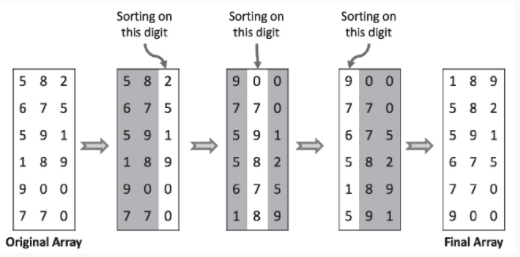
\includegraphics[width=1\columnwidth]{IEEEtran/radix.png}
    \caption{Exemplo de execução do algoritmo Radix-Sort}
    \label{fig:radix}
\end{figure}

Como exemplificado na Figura \ref{fig:radix} o algoritmo \textit{radix-sort} primeiramente verifica o digito menos significado e ordena os números de acordo com os valores, nessa etapa  o algoritmo utiliza métodos de ordenação estáveis para realizar essa operação como o \textit{counting-sort} e o \textit{bucket-sort} com o objetivo de obter o melhor tempo de execução. No trabalho presente foi utilizado o método \textit{counting-sort} tanto na versão paralela e na versão sequencial.

\section{Solução do Problema}
\label{chapter:solucao}
\subsection{Sequencial}
Na literatura são citadas diversas formas de realizar a ordenação \textit{radix}. A forma escolhida para o presente trabalho é, como dito anteriormente, utilizando o algoritmo \textit{counting-sort}. Então, basicamente o algoritmo consiste em aplicar o algoritmo \textit{counting-sort} considerando apenas o digito menos significativo e em seguida redistribuir os resultados ordenados em cada processo


\begin{algorithm}
\caption{Radix-Sort}
\DontPrintSemicolon
\SetKwFunction{FMain}{Main}

\SetKwProg{Fn}{Function}{:}{\KwRet}
 
  \SetKwProg{Fn}{Function}{:}{\KwRet}
  \Fn{\FMain}{
        $array = arrayInitialization()$\;
        \For{$j = 1 \rightarrow d $}{
            $ int count[10] = {0}\;$
            \For{$i = 0 \rightarrow n$}{
            $count[key of(A[i]) in pass j]++$
            }
            \For{$k = 1 \rightarrow 10$}{
            $count[k] = count[k] + count[k-1]$
            }
            \For{$i = n-1 \rightarrow 0$}{
            $result[ count[key of(A[i])] ] = A[j]$
                $count[key of(A[i])]--$
            }
            
            \For{$i=0 \rightarrow n$}{
            $A[i] = result[i]$
            }
        }
        \KwRet 0\;
  }
\end{algorithm}


\subsection{Paralelo}

A implementação da versão paralela foi inspirada na versão implementada por Yourii Martiak\footnote{$https://github.com/ym720/p\_radix\_sort\_mpi$}, ela foi levemente adaptada para os objetivos deste trabalho e é apresentado a seguir.

\begin{algorithm}
\caption{Radix-Sort-Paralelo}
\DontPrintSemicolon
\SetKwFunction{FMain}{Main}
\SetKwProg{Fn}{Function}{:}{\KwRet}
  \SetKwProg{Fn}{Function}{:}{\KwRet}
  \Fn{\FMain}{
        $MPI\_INIT()$\;
        \For{$i = 1 \rightarrow digit$}{
            $bucket-sort(array_local_cada_processo)$
            $distribuir\_dados\_entre\_processos()$
        }
        $MPI\_FINALIZE()\;$
  }
\end{algorithm}


Diferentemente da versão sequencial a versão paralela possui $N$ processos e cada processo será responsável por ordenar os valores de um sub-vetor que foi dividido para cada processo. Para cada digito dos valores existentes no \textit{array} a ser ordenado o algoritmo de ordenação percorre do digito menos significativo ao mais significativo entretanto antes de passar para o digito seguinte é feita uma distribuição dos dados entre os processos da forma que os os valores fiquem ordenados pelo numero e ordem de ocorrência, como exemplificado na Figura 

\begin{figure}[b]
    \centering
    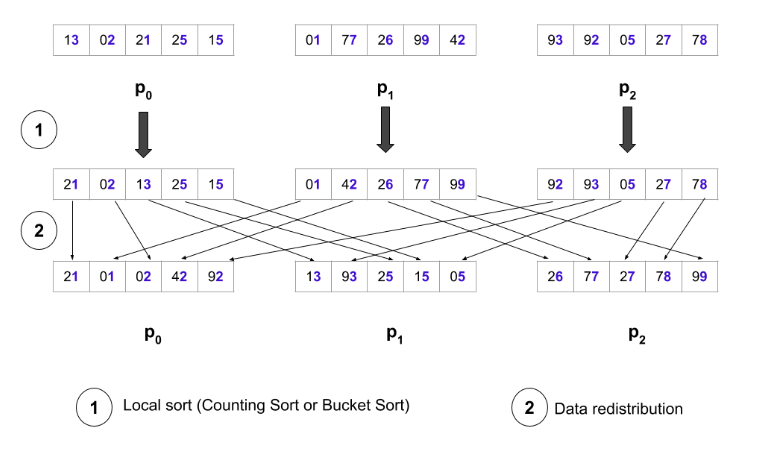
\includegraphics[width=1.0\linewidth]{IEEEtran/funcionamento.png}
    \caption{Funcionamento do algoritmo radix-sort paralelo.}
    \label{fig:radix-paralel}
\end{figure}


\section{Metodologia}
\label{chapter:metodologia}


Para obter os resultados e respostas acerca dos experimentos que serão apresentados nesse trabalho, foi utilizado a biblioteca \textit{sys/time.h}, que possui funções de marcação de tempo, disponível na linguagem C. Com o uso do tempo do sistema e das funções essa biblioteca foi coletado a principal informação que é o tempo de execução de cada execução, que com alguns cálculos podemos obter o \textit{speedup}.

\subsection{Ambiente}
Foi utilizado para a realização dos experimentos uma maquina com o S.O. Ubuntu 20.04 LTS,processador Intel Core i5-10210U com quatro núcleos físicos, com frequência base de 1.60 GHz e máxima de 4.20 GHz com 6Mb de cache e uma memória RAM de 8 Gbytes;

\subsection{Experimentos Realizados}

Foi pensando um modelo de teste que possui três tamanhos de entrada onde a maior possui $2^28$ elementos, a média possui $2^26$ e a menor possui $2^24$. Com isso, cada algoritmo, sequencial e paralelo, foi executado dez vezes para cada entrada sendo que o algoritmo paralelo possui uma nova variável: o número de processadores, que foi alternada entre dois e quatro. Foram realizados também experimentos com os mesmos valores onde não foram computados o tempo de inicialização, coleta dos dados e comunicação entre processos, foi apenas mensurada a computação paralela útil do programa.
Para obter uma melhor confiabilidade dos dados obtidos foi retirado o primeiro deles e realizado uma média simples dos nove valores restantes. 


\section{Análise e Discussão}
\label{chapter:analise}
\subsection{Speedup}

O \textit{SpeedUp}, ou fator de aceleração, é uma medida que relaciona a aceleração obtida por um algoritmo paralelo com o melhor algoritmo sequencial disponível para a execução da uma mesma tarefa. Matematicamente, o \textit{Speedup} corresponde à razão entre o tempo gasto na computação de um dado problema utilizando-se de apenas um processador e o corresponde à razão entre o tempo gasto na computação de um dado problema utilizando-se de \textit{p} processadores
\begin{equation}
S(t) = \frac{Tempo\ Sequencial}{Tempo\ Paralelo\ com\ n\ processadores}   
\end{equation}

\begin{figure}[htb]
    \centering
    \includegraphics[width=1.0\linewidth]{IEEEtran/speedup_small.png}
    \caption{Gráfico de \textit{SpeedUp}.}
    \label{fig:speedup}
\end{figure}


O \textit{radix sort} pode ser executado em tempo $O(nw)$, onde $n$ é o número de elementos da entrada e $w$ é a quantidade de dígitos que os elementos possuem. Em outras palavras, o \textit{radix sort} possui maior desempenho quando a entrada possui números com menor quantidade de dígitos.

Pode-se notar que no Figura \ref{fig:speedup} o desempenho do algoritmo paralelo quando analisado o gráfico de \textit{SpeedUp} não segue a teoria, comportamento linear, visto que esse comportamento teórico não considera as questões do S.O e do \textit{hardware}, ignorando o tempo de comunicação entre processos e do \textit{hardware}.
Pode-se perceber também que o \textit{speedup} dos algoritmos foi abaixo de um, indicando que possuem desempenho menor que o sequencial. Isso ocorre devido ao grande número de envio de dados entre os processadores, enviando cada valor separadamente. 
%Uma solução para esse problema seria juntar todos os elementos que precisam ser enviados à outros processadores e utilizar uma única comunicação, o que não foi realizado nesse trabalho devido às dificuldades encontradas durante o desenvolvimento. % revisar

Por outro lado, os algoritmos marcados com \textit{(p)} não contemplam o tempo de comunicação e de inicialização dos algoritmos, o que aumenta consideravelmente o \textit{speedup}, sendo quase linear para execução com dois processadores. 

\section{Considerações finais e trabalhos futuros}
\label{chapter:conclusao}

Como pode-se concluir, os resultados alcançados não são muito desejáveis, isso ocorre devido à grande quantidade de comunicações entre processos e \textit{delay} do próprio hardware. Temos resultados próximos ao ideal (linear) somente quando o algoritmo é executado com até 2 \textit{processos}, desconsiderando o tempo de comunicação e inicialização das variáveis. 

Como trabalhos relacionados pode-se apresentar o "\textit{Radix Sort For Vector Multiprocessors}"\cite{radixForVectorMultiprocessors1991Zagha_Blelloch} "Engineering a Multi-core Radix Sort" \cite{wassenberg2011engineering}
 

\ifCLASSOPTIONcaptionsoff
  \newpage
\fi

\nocite{*}

\bibliographystyle{IEEEtran}
\bibliography{bibliography.bib}
 
%\newpage



\end{document}


